%Comment this line out to use real graphics instead of demo boxes.
%Do not use \usepackage[demo]{graphicx} because that causes
%conflicts with other packages with dependencies.
\documentclass[sensors,article,submit,moreauthors,pdftex]{Definitions/mdpi} 
% If you would like to post an early version of this manuscript as a preprint, you may use preprint as the journal and change 'submit' to 'accept'. The document class line would be, e.g., \documentclass[preprints,article,accept,moreauthors,pdftex]{mdpi}. This is especially recommended for submission to arXiv, where line numbers should be removed before posting. For preprints.org, the editorial staff will make this change immediately prior to posting.

%--------------------
% Class Options:
%--------------------
%----------
% journal
%----------
% Choose between the following MDPI journals:
% acoustics, actuators, addictions, admsci, aerospace, agriculture, agriengineering, agronomy, algorithms, animals, antibiotics, antibodies, antioxidants, applsci, arts, asc, asi, atmosphere, atoms, axioms, batteries, bdcc, behavsci , beverages, bioengineering, biology, biomedicines, biomimetics, biomolecules, biosensors, brainsci , buildings, cancers, carbon , catalysts, cells, ceramics, challenges, chemengineering, chemistry, chemosensors, children, cleantechnol, climate, clockssleep, cmd, coatings, colloids, computation, computers, condensedmatter, cosmetics, cryptography, crystals, dairy, data, dentistry, designs , diagnostics, diseases, diversity, drones, econometrics, economies, education, electrochem, electronics, energies, entropy, environments, epigenomes, est, fermentation, fibers, fire, fishes, fluids, foods, forecasting, forests, fractalfract, futureinternet, futurephys, galaxies, games, gastrointestdisord, gels, genealogy, genes, geohazards, geosciences, geriatrics, hazardousmatters, healthcare, heritage, highthroughput, horticulturae, humanities, hydrology, ijerph, ijfs, ijgi, ijms, ijns, ijtpp, informatics, information, infrastructures, inorganics, insects, instruments, inventions, iot, j, jcdd, jcm, jcp, jcs, jdb, jfb, jfmk, jimaging, jintelligence, jlpea, jmmp, jmse, jnt, jof, joitmc, jpm, jrfm, jsan, land, languages, laws, life, literature, logistics, lubricants, machines, magnetochemistry, make, marinedrugs, materials, mathematics, mca, medicina, medicines, medsci, membranes, metabolites, metals, microarrays, micromachines, microorganisms, minerals, modelling, molbank, molecules, mps, mti, nanomaterials, ncrna, neuroglia, nitrogen, notspecified, nutrients, ohbm, particles, pathogens, pharmaceuticals, pharmaceutics, pharmacy, philosophies, photonics, physics, plants, plasma, polymers, polysaccharides, preprints , proceedings, processes, proteomes, psych, publications, quantumrep, quaternary, qubs, reactions, recycling, religions, remotesensing, reports, resources, risks, robotics, safety, sci, scipharm, sensors, separations, sexes, signals, sinusitis, smartcities, sna, societies, socsci, soilsystems, sports, standards, stats, surfaces, surgeries, sustainability, symmetry, systems, technologies, test, toxics, toxins, tropicalmed, universe, urbansci, vaccines, vehicles, vetsci, vibration, viruses, vision, water, wem, wevj

%---------
% article
%---------
% The default type of manuscript is "article", but can be replaced by: 
% abstract, addendum, article, benchmark, book, bookreview, briefreport, casereport, changes, comment, commentary, communication, conceptpaper, conferenceproceedings, correction, conferencereport, expressionofconcern, extendedabstract, meetingreport, creative, datadescriptor, discussion, editorial, essay, erratum, hypothesis, interestingimages, letter, meetingreport, newbookreceived, obituary, opinion, projectreport, reply, retraction, review, perspective, protocol, shortnote, supfile, technicalnote, viewpoint
% supfile = supplementary materials

%----------
% submit
%----------
% The class option "submit" will be changed to "accept" by the Editorial Office when the paper is accepted. This will only make changes to the frontpage (e.g., the logo of the journal will get visible), the headings, and the copyright information. Also, line numbering will be removed. Journal info and pagination for accepted papers will also be assigned by the Editorial Office.

%------------------
% moreauthors
%------------------
% If there is only one author the class option oneauthor should be used. Otherwise use the class option moreauthors.

%---------
% pdftex
%---------
% The option pdftex is for use with pdfLaTeX. If eps figures are used, remove the option pdftex and use LaTeX and dvi2pdf.

%\documentclass[preprint,sort&compress]{elsarticle}
\usepackage{amsmath}
\usepackage[version=3]{mhchem}
\usepackage{url}
\usepackage{graphicx}
\usepackage{threeparttable}
\usepackage{pdfpages}
\usepackage{multirow}
\usepackage{siunitx}
\usepackage{microtype}
\usepackage{placeins}
\newcommand{\degree}{$^{\circ}$}

\firstpage{1} 
\makeatletter 
\setcounter{page}{\@firstpage} 
\makeatother
\pubvolume{xx}
\issuenum{1}
\articlenumber{5}
\pubyear{2019}
\copyrightyear{2019}
%\externaleditor{Academic Editor: name}
\history{Received: date; Accepted: date; Published: date}
%\updates{yes} % If there is an update available, un-comment this line

\graphicspath{ {./images/} } %this removes clutter from the root folder

% Full title of the paper (Capitalized)
\Title{Precision and Limits of Detection for Selected Commercially Available, Low-cost Carbon Dioxide and Methane Gas Sensors}

% Author Orchid ID: enter ID or remove command
\newcommand{\orcidauthorA}{0000-0002-3681-4810} % Add \orcidA{} behind the author's name
\newcommand{\orcidauthorB}{0000-0003-4266-5011} % Add \orcidB{} behind the author's name
%\newcommand{\orcidauthorC}{0000-0003-4266-5011} % Add \orcidC{} behind the author's name

% Authors, for the paper (add full first names)
\Author{Wesley T. Honeycutt $^{1,\dagger,}$\orcidA{}, M. Tyler Ley $^{2,}$, and Nicholas F. Materer $^{3,}$\orcidB{}*}

% Authors, for metadata in PDF
\AuthorNames{Wesley T. Honeycutt, M. Tyler Ley, and Nicholas F. Materer}

% Affiliations / Addresses (Add [1] after \address if there is only one affiliation.)
\address{%
	$^{1}$ \quad Oklahoma State University, Department of Chemistry, 107 Physical Sciences, Stillwater, OK 74078, USA; wes.honeycutt@okstate.edu \\
	$^{2}$ \quad Oklahoma State University Department of Civil Engineering; 319C Engineering South, Stillwater, OK 74078, USA; tyler.ley@okstate.edu \\
	$^{2}$ \quad Oklahoma State University Department of Chemistry; 107 Physical Sciences, Stillwater, OK 74078, USA; materer@okstate.edu
}%

% Contact information of the corresponding author
\corres{Correspondence: materer@okstate.edu}

% Current address and/or shared authorship
\firstnote{Current address: University of Oklahoma Biological Survey; 111 Chesapeake St.; Norman, OK 73019, USA} 
%\secondnote{These authors contributed equally to this work.}
% The commands \thirdnote{} till \eighthnote{} are available for further notes

\abstract{%
	The performance of a sensor platform for environmental or industrial monitoring is sensitive to the cost and performance of the individual sensor elements.
	%
	Thus, the detection limits, accuracy, and precision of commercially available, low-cost carbon dioxide and methane gas concentration sensors were evaluated by precise measurements at known gas concentrations.
	%
	Sensors were selected based on market availability, cost, power consumption, detection range, and accuracy.
	%
	A specially constructed gas mixing chamber, coupled to a precision bench-top analyzer, was used to characterize each sensor during a controlled exposure to known gas concentrations.
	%
	For environmental monitoring, the selected carbon dioxide sensors were characterized around 400 ppm.
	%
	For the methane, sensor response was first monitored at 0 ppm, close to the typical environmental background.
	%
	The selected sensors were then evaluated at gas concentrations up to 1000 ppm.
	%
	The determined detection limits accuracy, and precision provides a set of matrices that can be used to evaluate and select sensors for integration into a sensor platform for specific applications.
}%

\keyword{Sensor systems and applications, Carbon Dioxide, Methane}

\begin{document}
	
	\section{Introduction}
	\label{sec:intro}
		
		Environmental monitoring of local gas concentration is becoming increasingly important to ensure worker safety and for early identification of potential leaks.
		%
		Sensor platforms for real time monitoring of carbon dioxide and methane gas concentrations are of interest as these gases can impact animal health and crop growth.
		%
		Since these gases are also considered greenhouse gases, monitoring of industrial sites is important to understand their impact on the environment.
		%
		Collection of multiple samples at multiple locations in a given area is critical to obtain reliable results, and this directly impacts the overall complexity and cost.
		%
		Aspects of effective sampling, along with other considerations, are discussed by Keith et al.~\cite{keith_principles_1983}.
		%% PARA
		
		Potential sensor platforms must consider the limit of detection, precision, accuracy, reliability, and power consumption for each sensor integrated within the unit.
		%
		Such devices include, but are not limited to, those used in HVAC air handlers~\cite{yang_systematic_2014,chung_selective_2008}, chemical processing units~\cite{won_nonlinear_2012}, oil well monitoring devices~\cite{yi_remote_2010,somov_deployment_2013}, and environmental monitoring~\cite{pering_high_2014,black_formation_2012,guohua_study_2012,karunanithi_performance_2009,shendell_outdoor_2012}.
		%
		Given the large number of commercially available sensors and papers discussing their use in various applications, there is limited literature that directly compares the precision, sensitivity and limits of detection of the sensor elements.
		%
		This lack of information hinders one's ability to select the optimal sensors for sensor platform designed for a given application.
		%
		To address this issue, an array of commercially available, low-cost sensors for carbon dioxide (CO$_2$) and methane (CH$_4$) were evaluated at concentrations typical to those required for environmental monitoring, and monitoring around carbon sequestration operations and oil fields.
		%% PARA
		
		Low-cost sensors currently available can be generally categorized by detection method.
		%
		Principal among these methods are optical absorption, chemiresistive (based on the electrical changes due to a chemical reaction with an analyte~\cite{wetchakun_semiconducting_2011}), and electrochemical.
		%
		Since studies have cited concerns with electrochemical sensors, such as a short lifetime and lack of robustness~\cite{neri_first_2015}, only optical and chemiresistive sensors were selected for evaluation in this study.
		%
		Optical methods of detecting carbon dioxide and methane are based on measuring the absorption of light at \SI{2352}{\per\centi\meter} and \SI{3015}{\per\centi\meter}, respectively~\cite{frodl_high-precision_2006,zhu_one_2012}.
		%
		Since these sensors utilize the Beer-Lambert law to relate absorption to concentration, the calibration is only dependent on the geometry of the sensor and physical properties of the gas~\cite{bacsik_ftir_2004}.
		%% PARA
		
		Lower cost optical sensors typically utilize nondispersive infrared (NDIR) sensing.
		%
		This method utilizes a broad spectrum source of light which is restricted by a narrow band pass filter across the absorbance maximum before reaching the detector.
		%
		As a result, lower cost parts can be used and the design can be both more compact and robust.
		%
		In general, NDIR detection is utilized for carbon dioxide due to its relatively large molar absorption coefficient, allowing for short path lengths to be used in devices.
		%
		Methane is limited in practical applications due to its lower absorption coefficient and overlapping symmetric C-H stretches.
		%
		The overlapping stretches makes methane difficult to distinguish from other common aliphatic gases such as ethane and propane~\cite{coblentz_society_inc._evaluated_????}.
		%
		Although selectivity of the NDIR sensors with respect to different analyte gases was not explored in this study, it should be considered when these sensors are integrated into a monitoring device. 
		%% PARA
		
		Chemiresistive sensors for detection of methane typically use a thin oxide film~\cite{neri_first_2015}.
		%
		These sensors work by measuring resistance changes due to differences in the electron transport through the metal oxide film, in the presence of oxygen and reactive gases~\cite{albert_cross-reactive_2000}.
		%
		When the film is exposed to methane, the molecule adsorbs and reacts with surface oxygen species resulting in a change in the electrical conductivity~\cite{wang_metal_2010,prudenziati_thick-film_1986}.
		%
		Since the sensor depends on chemical reactions involving both atmospheric oxygen and methane for proper functioning, the measurement is dependent on the relative humidity, temperature, and film preparation.
		%
		Chemiresistive sensors are also known to respond to a range of hydrocarbon gases~\cite{sekhar_development_2016}. In many cases, the non-linear response curves for additional gases are included in the documentation provided by the manufacturer.
		%
		However, similar to the optical sensors for methane, the selectivity was not explored but should be considered when integrating these sensors into a sensor platform.
		%% PARA
		
	\section{Methods}
		\label{sec:methods}
		
		\subsection{Sensor Selection}

			With two exceptions, the sensors selected were all commercially available in large volumes (at least 1000 units) at low-cost (defined here as less than \$100 per unit in bulk)
			%
			Selected sensors were expected to have sensitivity at the environmental concentrations of carbon dioxide and methane.
			%
			For carbon dioxide, this level is around 400 ppm~\cite{blasing_recent_2016,dlugokencky_trends_2016}.
			%
			For methane, the baseline atmospheric concentration is under 2 ppm~\cite{turner_large_2016,bamberger_spatial_2014,dlugokencky_trends_2016-1}.
			%
			In total, six carbon dioxide sensors were selected for testing, the K-30 SE-0018, COZIR AMB GC-020, Gascard CO$_{2}$, MSH-P/CO2/NC/5/V/P/F, MSH-DP/HC/CO2/NC/P/F, and Telaire T6615.
			%
			Given the prevalence of optical sensors for carbon dioxide, no chemiresistive sensor was selected for this analyte.
			%
			For methane, seven sensors were evaluated, the MQ-4, Gascard CH$_{4}$, MSH-P/HC/NC/5/V/P/F, MSH-DP/HC/CO2/NC/P/F, TGS-2600, TGS-2610, and TGS-2611.
			%
			The relevant properties, obtained from the manufacturer documentation, for the carbon dioxide (Table S1) and methane sensors (Table S2) are summarized in the supplementary materials.
			%
			The selected sensors meet the requirements for use in portable low-power monitoring devices~\cite{karpov_energy_2013}.
			%% PARA
			
			The K-30, COZIR, Dynament, and Telaire sensors are all NDIR carbon dioxide sensors.
			%
			The Dynament hydrocarbon sensor (MSH-P/HC) was chosen as inexpensive candidates for methane detection.
			%
			Dynament also provides a dual gas NDIR sensor (MSH-DP/HC/CO2) designed to measure both carbon dioxide and methane concentrations, which is attractive for applications requiring both low-cost and portability.
			%
			Finally, carbon dioxide and methane Gascard (sold by GHG Analytical) sensors were included, even though they were more expensive than the other chosen NDIR sensors.
			%
			 However, the Gascard sensors are still significantly less expensive than typical bench-top instruments. The inclusion of pressure and temperatures compensation make them attractive enough to compensate for the expense.
			%% PARA
			

			The low-cost chemiresistive-based methane sensors studied here are typically used in gas warning systems~\cite{chiu_towards_2013}.
			%
			Selected sensors include the MQ-4 from Hanwei Electronics and TGS-2600, TGS-2610, and TGS-2611 manufactured by Figaro Engineering Inc. sensors.
			%
			The TGS sensors are used in commercial methane detectors, and the TGS-2600 sensor has been previously evaluated for atmospheric applications~\cite{eugster_performance_2012,bossche_potential_2017}.
			%
			There are several different MQ versions optimized for hydrocarbon sensing.
			%
			The MQ-4 sensor was chosen as this variant was specifically tuned for methane.
			%
			Chemiresistive sensors required a minimum conditioning period or ``burn-in'' time.
			%
			The ``burn-in'' time was met or exceeded for all chemiresistive sensors.
			%% PARA
			
		\subsection{Analyte Preparation and Sensor Testing}
			
			To test these sensors under controlled conditions, a gas mixing apparatus (Fig.~\ref{fig:exposureapparatus}) was constructed.
			%
			A high-quality bench-top analyzer (California Analytical Instruments, Inc. ZRE Non-Dispersive Infrared Analyzer), sensitive to both carbon dioxide and methane, was used as a precision reference. This setup allows gas flows of a known concentration to be prepared from a calibrated gas cylinder by mixing with a carrier gas.
			%
			The calibrated gas contained a mixture of gases at concentrations listed in Table~\ref{tab:ratios} depending on the specific experiment being performed.
			%
			Since the objective is to address the accuracy, precision, sensitivity, and limits of detection, only carbon dioxide and methane were utilized.
			%
			However, selectivity requirements must be considered when these sensors are integrated into a monitoring platform.
			%
			For carbon dioxide experiments, the carrier gas was typically nitrogen.
			%
			For methane, medical grade air was utilized since the chemiresistive sensors required oxygen to correctly measure the methane concentration.
			%
			All reported concentrations were determined using the bench-top analyzer.
			%
			Thus, the concentration ranges and all reported values are not whole numbers.
			%% PARA
			
			\begin{figure}[!t]
				\centering
				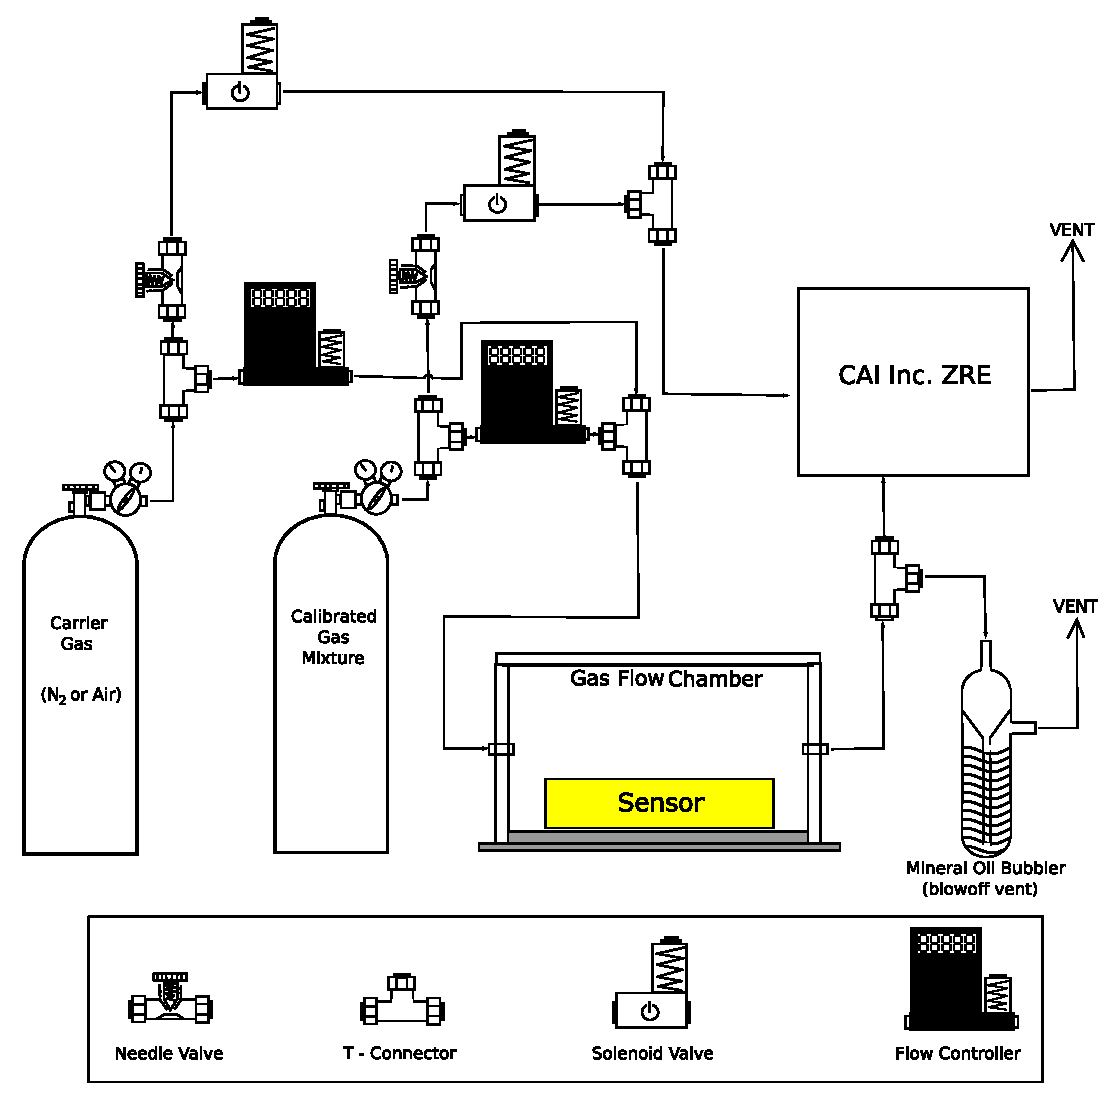
\includegraphics[width=\columnwidth]{honey1.pdf}
				\caption{Component diagram of controlled gas exposure apparatus with chamber for diffusion-type sensors.}
				\label{fig:exposureapparatus}
			\end{figure}
				
			\begin{table}[!t]
				\caption{Calibrated gas mixtures used to prepare various gas mixtures with a carrier gas.}
				\label{tab:ratios}
				\small
				\centering
				\begin{tabular}{c | c | c}
					Carbon Dioxide & Methane  & Balance Gas \\ \hline
					3000 ppm       & 3000 ppm & nitrogen    \\
					100 ppm        & 100 ppm  & nitrogen    \\
					0 ppm          & 20 ppm   & nitrogen
				\end{tabular} 
			\end{table}
			
			The calibrated gas mixtures were provided by and certified within $\pm$2\% by Airgas Inc.
			%
			The calibrated gas was diluted using either air or nitrogen gas by a set of mass flow controllers to produce specific concentration of the analyte gases.
			%
			The solenoid valves in the gas mixing apparatus were used to send either the undiluted calibrated gas or the carrier gas to analyzer for calibration purposes.
			%
			This ability allows the analyzer to be periodically calibrated.
			%
			The uncertainty in the gas concentration results in a systematic error.
			%
			Around atmospheric levels of methane, this error is less than 0.4~ppm.
			%
			For atmospheric levels of carbon dioxide, the error is approximately 8~ppm.
			%
			Since the fluctuations around the mean were independent of the exact concentration (see Section~\ref{sec:main_baseline}), this systematic error will not affect the results from the baseline noise or the International Union of Applied Chemistry (IUPAC) Limit of Detection, discussed below.
			%
			For the sensor calibrations, uncertainty in the absolute concentration of the carrier gas will introduce an error in the intercept but not the slope.
			%
			Thus, this systematic error will have small effect on the calibration-corrected Limit of Detection.
			%
			However, this systematic error was found to be insignificant relative to the random errors in the experiment.
			%% PARA
			
			Multiple sensors were operated concurrently as shown in Fig.~\ref{fig:exposureapparatus2}.
			%
			The ``Gas Mixer'' in this diagram is the gas mixing apparatus shown in Fig.~\ref{fig:exposureapparatus}, and the ``Gas Analyzer'' is the California Analytical Instruments, Inc. ZRE Non-Dispersive Infrared Analyzer.
			%
			There are two types of sampling methods used by the selected sensors; diffusion and flow (see Table S1 and S2 in the supplemental).
			%
			Flow sampling sensors are designed such that the analyte gases must physically pass through a sampling chamber within the sensor.
			%
			In terms of applications, these sensors typically require additional filters to be added upstream to prevent inclusion of particulate matter, which may damage the sensor or introduce measurement error.
			%
			In the experimental setup (Fig.~\ref{fig:exposureapparatus2}), the flow capable sensors were connected directly to gas flow from the mixing apparatus.
			%
			In addition to the flow sensors, another common sampling technique relies on diffusion through a fine mesh screen or film.
			%
			The diffusion method allows the sensing element to be exposed to the analyte gas while still being protected from particulate contaminants.
			%
			This method also eliminates the extra pump and particulate filters required for sensors that require gas flow.
			%
			The small ``sensor flow box'' enclosures depicted in Fig.~\ref{fig:exposureapparatus2} contained the K-30 carbon dioxide sensor and a socketable chemiresistive methane sensor (such as the MQ-4 or TGS series sensors).
			%
			The larger ``gas flow chamber'' contained the COZIR, Telaire, Dynament, and K-30 sensors.
			%
			Given the large total volume, data collected from the sensors in this chamber were analyzed only after the system reached a constant concentration following the introduction of a gas with known concentration of carbon dioxide or methane.
			%
			In some experiments, performed to accurately measure the response time for chemiresistive sensors, a smaller sensor enclosure (internal volume \SI{2.54}{\centi\meter\cubed}) was used to minimize the time to reach a stable concentration.
			%% PARA
			
			
			\begin{figure}[!t]
				\centering
				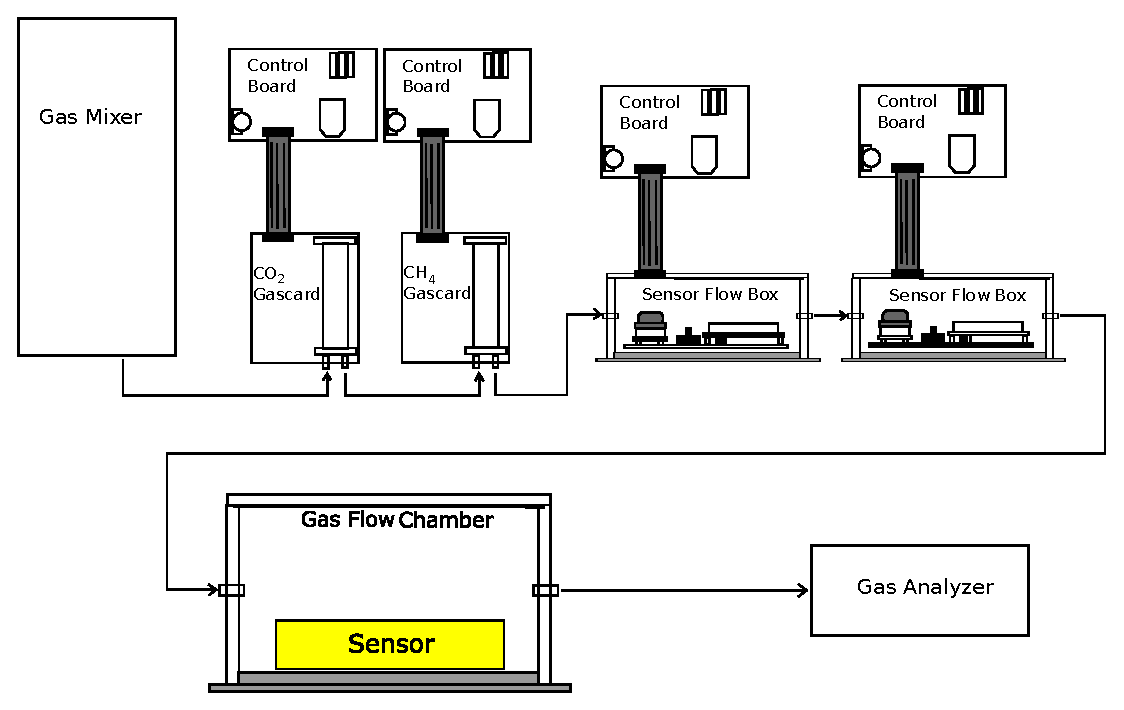
\includegraphics[width=\columnwidth]{honey2.pdf}
				\caption{The diagram shows the flow of gas from the mixing apparatus to Gascard sensors, small enclosures containing sensors, the large gas flow chamber, and finally to the California Analytical Instruments, Inc. ZRE Non-Dispersive Infrared Analyzer.
				%
				The gas mixing apparatus is shown in Fig.~\ref{fig:exposureapparatus}.
				%
				The reported concentrations are based on the value detected by the California Analytical Instruments, Inc. ZRE Non-Dispersive Infrared Analyzer.}
				\label{fig:exposureapparatus2}
			\end{figure}
			
		\subsection{Sensor Output and Data Collection}
		\label{sec:method_data}
		
			\begin{equation}
				\label{eq:vtos}
				\varsigma = \frac{V_{measured}}{V_{cc}-V_{measured}}\times \frac{1}R_{ref}\\
			\end{equation}
			
			The output of each sensor was logged as a function of time using software provided by the manufacturer as part of development kits when provided, or using an Arduino microcontroller with a prototyping board and microSD card.
			%
			Due to the unique interface requirements of each sensor, development kits were purchased when possible.
			%
			In all cases, the internal electronics within the selected optical sensors process the option data and provide a digital output.
			%
			For example, the K-30 reports the concentration directly, while the Gascard reports a digital value between zero and one, with one being the maximum concentration (30,000 ppm carbon dioxide for the sensor used in this study).
			%
			For the Gascard, the scaling was applied to the output before analyzing.
			%
			The chemiresistive sensors were energized using the recommended voltage for the heater element and the response was measured using a 12-bit A/D converter, after buffering and filtering, across a reference resistor (a 10 k$\Omega$ resistor was used for $R_{ref}$).
			%
			The A/D converter was referenced using the 5V supply, which was also connected to the sensing element of the chemiresistive sensor. Equation~\ref{eq:vtos} describes the conversion of the measured voltage ($V_{measured}$) to the conductivity ($\varsigma$), measured in Siemens (S).
			%% PARA
			
	
		\subsection{Calibration and Fitting Procedures}
			\label{sec:method_cal}
			
			Calibration curve of each sensor was determined by varying concentrations and recording the output with time.
			%
			The carbon dioxide sensors were calibrated using gas concentrations from 34.5 to 1020 ppm.
			%
			For the methane sensors, calibration curves were generated from gas concentrations between 1.85 and 995 ppm.
			%
			 The procedure starts with a constant flow of the carrier gas until stable baseline is obtained.
			%
			Next, the analyte gas at a known concentration is introduced.
			%
			After 24 hours, the carrier gas is reintroduced and the system is again allowed to stabilize before the next measurement. During this procedure, concentration data from each sensor was continually collected. From this data, the average baseline and response to each gas concentration can be extracted.
			%
			The average response at each concentration was determined from the data collected after the system stabilized (include any overshoot or ringing) after each new concentration.
			%% PARA
			
			\begin{equation}
				\label{eq:langmuirian}
				f(x)=\frac{a\times b\times x}{1+b\times x}
			\end{equation}

			The fitting procedures for the optical and chemiresistive sensor differ.
			%
			The raw output of the optical absorption-based sensors is expected to follow Beer-Lambert law.
			%
			In all cases, the internal electronics within the selected optical sensors process the absorbance and provide a digital output.
			%
			For the optical sensors, the accuracy and precision of the internal calibration are quantified by linear regression.
			%
			The calibration curves for the chemiresistive are non-linear, and modeled using a Langmuir-like or Langmuirian form (Equation~\ref{eq:langmuirian}). Equation~\ref{eq:langmuirian} converges to a linear function the ppm approaches zero, which simplifies the Limit of Detection calculations discussed below.
			%
			The parameters $a$ and $b$, along with the asymptotic standard errors, are determined by fitting the experimental data using the Levenberg-Marquardt algorithm in $gnuplot$~\cite{williams_gnuplot_2016}.
			%
			Additional non-linear functions have been suggested by kinetic analysis~\cite{barsan_fundamental_1999,ahlers_rate_2005}. Of these, a power law model, where the log of the output is proportional to the log of the ppm, is considered.
			%% PARA
			
		\subsection{Precision and Baseline Noise Tests}
			\label{sec:method_baseline}
		
			The precision of the sensors was determined by a 20- to 30-hour data collection run at a known concentration and uniform flow.
			%
			These experiments were performed around the baseline atmospheric concentration for each analyte gas, which is approximately 400 ppm for carbon dioxide~\cite{blasing_recent_2016,dlugokencky_trends_2016} and under 2 ppm for methane~\cite{turner_large_2016,bamberger_spatial_2014,dlugokencky_trends_2016-1}. 
			%% PARA
				
		
		\subsection{Limit of Detection Determination}
			\label{sec:method_detection}
			The Limit of Detection is the minimum concentration that can be detected as significantly different from the background~\cite{long_limit_1983,currie_detection:_1997,mocak_j._statistical_2009}.
			%
			IUPAC defines the Limit of Detection as three times the standard deviation ($\sigma$) from the background.
			%
			For the sensors discussed here, the raw output from the sensors must be transformed into concentration value, and any error in the calibration will affect the Limit of Detection.
			%
			For measurements requiring a calibration curve, Long and Winefordner provide a review of the various definitions as well as several examples~\cite{long_limit_1983}.
			%
			For optical sensors, their procedure to include the errors in the slope and intercept in the calculated the Limit of Detection was utilized.
			%
			For the non-linear chemiresistive sensors, the asymptotic standard errors in $a$ and $b$ were propagation to correct the IUPAC Limit of Detection.
			%% PARA
			
	
	\section{Results and Discussion}
	
		\subsection{Sensor Response}
		\label{sec:time}
	
			Fig.~\ref{fig:peakdetailco2} shows the response of two selected carbon dioxide sensors, the K-30 and Gascard, to 600 and 1400 concentration steps of carbon dioxide.
			%
			The K-30 output was used directly, while the Gascard data was multiplied by the provided scaling factor before plotting.
			%
			This data demonstrates relative similarity in behavior of the selected sensors in the presence of concentration changes well above the limit of detection.
			%
			It was observed that all the optical sensors responded quickly to an increase in carbon dioxide inside the environmental chamber, limited only by the internal sampling rate of the sensor.
			
			\begin{figure}[!t]
				\centering
				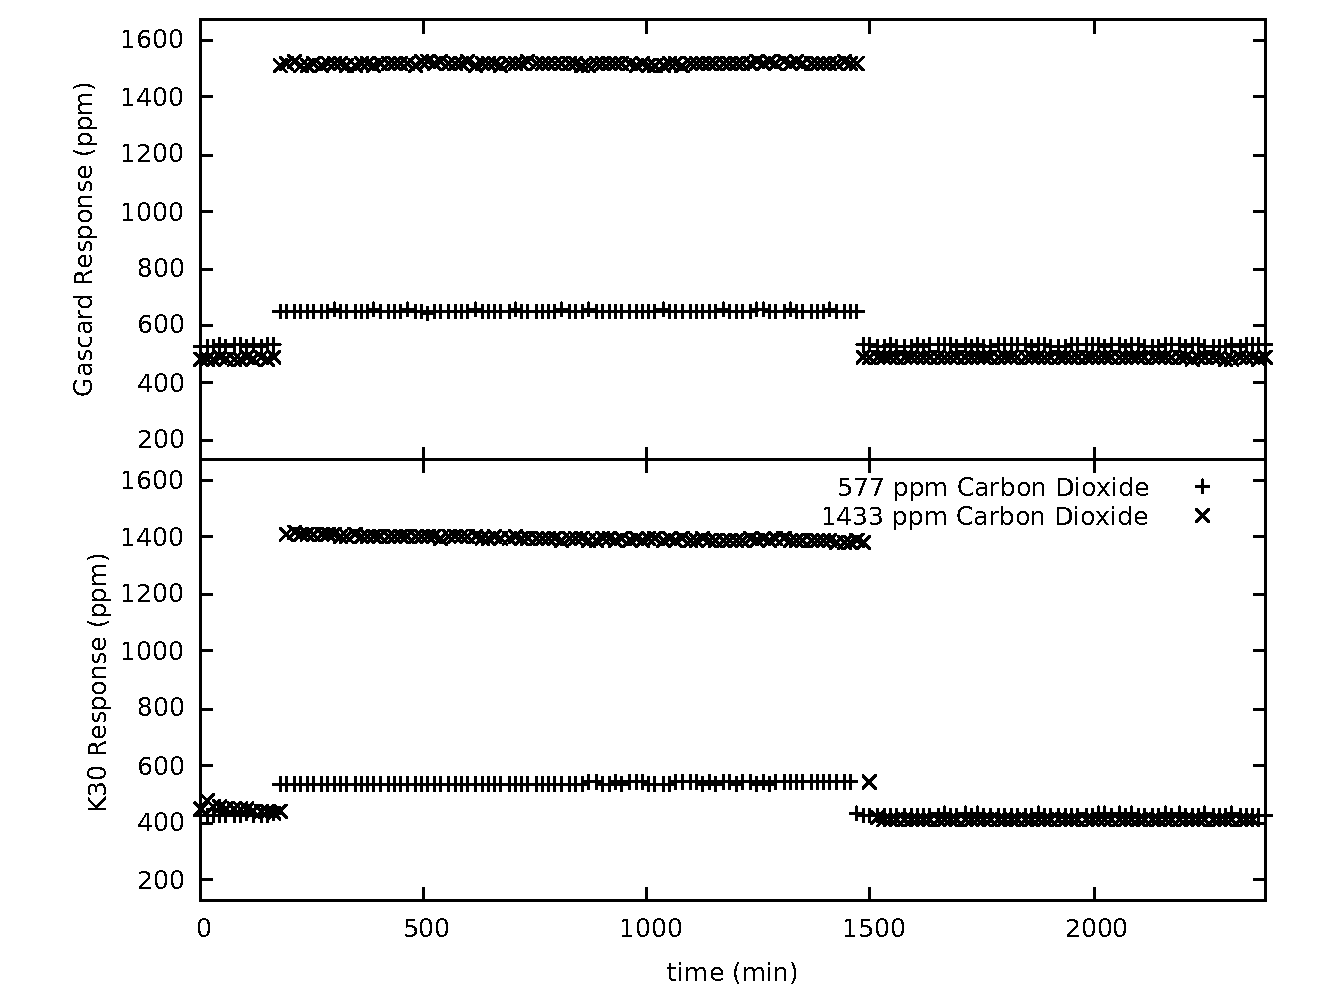
\includegraphics[width=\columnwidth]{honey3.pdf}
				\caption{The Gascard (top) and K-30 (bottom) sensor response over time at high (1433 ppm, plotted with ``$\times$'' on the plot) and low (577 ppm, plotted with ``$+$'') concentrations of carbon dioxide.
				%
				The reported concentrations (577 and 1433 ppm) were determined by the California Analytical Instruments, Inc. ZRE Non-Dispersive Infrared Analyzer.}
				\label{fig:peakdetailco2}
			\end{figure}
			
			Fig.~\ref{fig:mq4step} depicts a plot of the response of an MQ-4 sensor upon exposure to five different concentrations of methane between 500 and 2200 ppm, which could represent a methane leak. In our setup, the MQ-4 produces significant overshoot. Some of the overshoot is inherent to the sensor, but some could also be a result of the small interruption in the gas flow during a concentration change.
			%
			For all concentrations, a stable value within 2.5\% of the mean was produced after 78$\pm$\SI{10}{\second}, when averaged over all experiments.
			%
			The settling time for the MQ-4 sensor did not appear to be concentration dependent. Shorter settling time and less overshoot was observed for the TGS sensors.
			%% PARA
			
	
			\begin{figure}[!t]
				\centering
				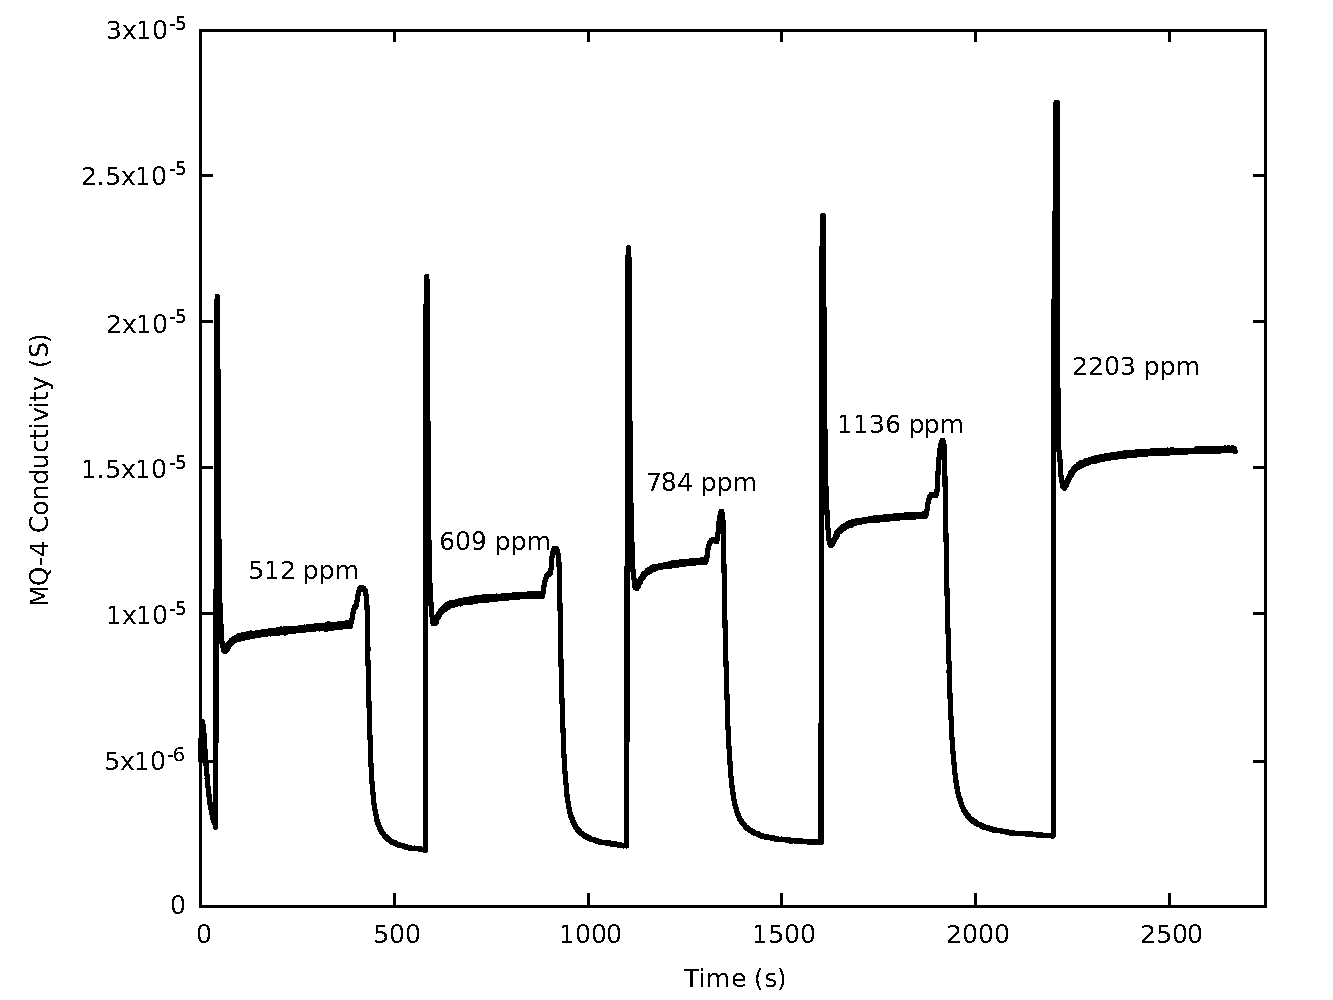
\includegraphics[width=\columnwidth]{honey6.pdf}
				\caption{The MQ-4 response to difference methane concentrations determined by the California Analytical Instruments, Inc. ZRE Non-Dispersive Infrared Analyzer.}
				\label{fig:mq4step}
			\end{figure}
			
		\subsection{Calibration Result}
			\label{sec:calibration}

			Typical calibration plots for an optical and a chemiresistive sensors are shown in Fig.~\ref{fig:gascardcodiff}.
			%
			The data points are the measured values at each concentration, while the line is a fit to the data.
			%
			The upper plot in Fig.~\ref{fig:gascardcodiff} is a calibration curve obtained from the Gascard sensor, along with the linear fit.
			%
			The slope is $1.02\pm 0.02$ indicating an excellent calibration and precision.
			%
			Above their respective detection limits, good linear fits were obtained for each optical sensor. Linear regression results show the slopes for the selected sensors are all close to one, indicting good precision.
			%
			For the carbon dioxide sensors, the slopes range from 1.11 to 0.86, with the MSH-P/CO2 and Telair as the high and low outliers, respectfully.
			%
			Excluding these sensors, the average slope is 0.99.
			%
			For the methane sensors, the slopes are 0.98 (Gascard), 1.03 (MSH-DP/HC/CO2), and 1.20 (MSH-P/HC).
			%
			The fact that a majority of the slopes are close to one is expected as the optical path length and the physical properties of the analyte determine the response.
			%
			In contrast to the slopes, the value of the vertical intercept or the response at zero concentration vary widely, exceeding several 100 ppm in many cases.
			%
			Large variations are found even between sensors from the same manufacture. Since the intercept depends on the intensity of the source and the detector, these variations are not unexpected.
			%
			To address this issue, a majority of the optical sensors tested provide an easy way to adjust the intercept.
			%
			For example, the K30 sensors can autocalibrate the zero based on known average background level of carbon dioxide.
			%
			In general, it was found the intercept must be adjusted before deployment.
			%% PARA
			
			\begin{figure}[!t]
				\centering
				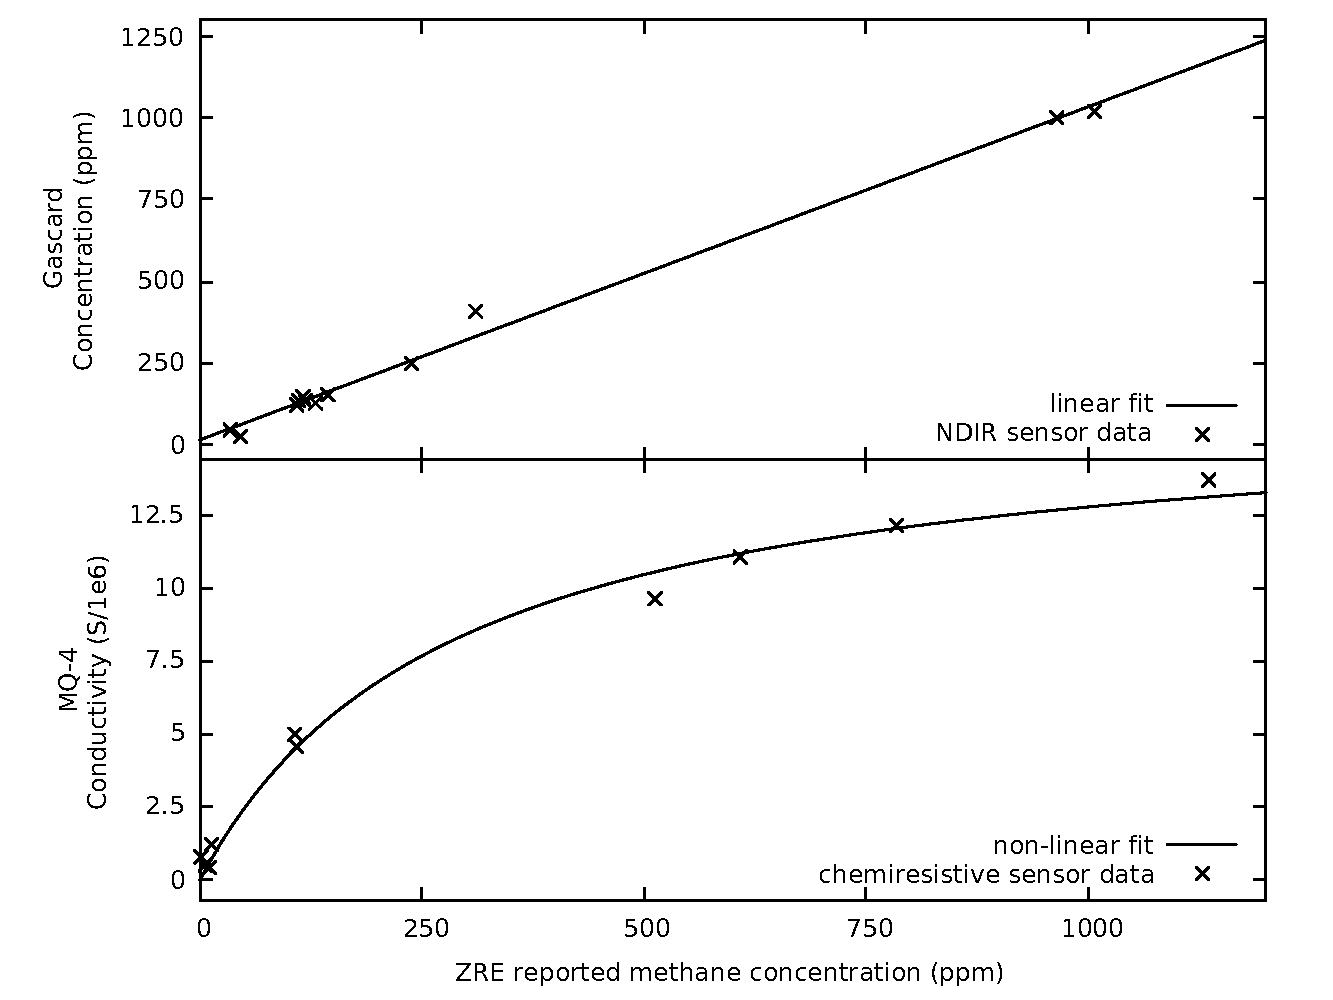
\includegraphics[width=0.9\columnwidth]{honey9.pdf}
				\caption{The response of the Gascard and MQ-4 sensors with respect to the concentration reported from the California Analytical Instruments Inc. ZRE Non-Dispersive Infrared Analyzer for different concentrations of either carbon dioxide or methane, respectively.
					%
					The top part of the figure shows the response of an optical carbon dioxide sensor with the expected linear behavior.
					%
					The bottom part of the figure shows the response of a chemiresistive methane sensor (MQ-4, response is expressed in conductivity) with a fit to the non-linear response}
				\label{fig:gascardcodiff}
			\end{figure}
			
			The lower plot in Fig.~\ref{fig:gascardcodiff} shows the response of a chemiresistive methane sensor (MQ-4, response is expressed in conductivity) with non-linear fit to a  Langmuirian form  (Equation~\ref{eq:langmuirian}).
			%
			For ppm concentration above 500 ppm, acceptable results were also obtained using a power law model. However, this model produced a fit that increased too rapidly with ppm at lower concentration.
			%
			At high concentrations, this model did not accurately represent a real sensor where the response approaches a constant.
			%
			A lower concentration reference gas was required to precisely prepare an analyte gas at 100 ppm and below.
			%
			This action resulted in a gap between 100 and 500 ppm in the lower plot.
			%
			It is also significant that the chemiresistive sensors shows a rapid increase in conductivity with concentration below 100 ppm when compared to the optical sensors.
			%% PARA
			
			Unlike optical sensors for carbon dioxide, which only needs reading at zero ppm to be experimentally established, chemiresistive sensors require the measurement of a complete non-linear calibration curve to ensure accuracy and precision.
			%
			The output of the chemiresistive sensors are also dependent on temperature and humidity, further complicating the calibration~\cite{benkstein_analytical_2014}.
			%
			Although the selected chemiresistive sensors have the requisite precision to provide a clear indication of a change (based on number of $\sigma$ above the noise, see Table~\ref{tab:stddev} along with the associated discussion below) at the ppm level, obtaining an accurate result is challenging.
			%% PARA
			

		\subsection{Precision and Baseline Noise Tests}
			\label{sec:main_baseline}
			
			The measurement precision and baseline noise of each sensor was performed as described in Section~\ref{sec:method_baseline}.
			%
			In most cases, the precision of the sensors was determined by a 20 to 30 hour data collection time at a known concentration (400 ppm for carbon dioxide and 0 ppm for methane based on previously discussed atmospheric baselines)under a uniform flow.
			%
			In general, the optical sensors displayed flat baselines. Chemiresistive sensors typically display baseline changes due to humidity and temperature, which must be taken into account in monitoring applications. Fig.~\ref{fig:MQ4TGSbaseline} shows a typical data set for the TGS-2611 and MQ-4 sensor.
			%
			TGS-2611 sensor displayed significantly less baseline drift than the MQ-4 sensor.
			%% PARA
			
			
			\begin{figure}[!t]
				\centering
				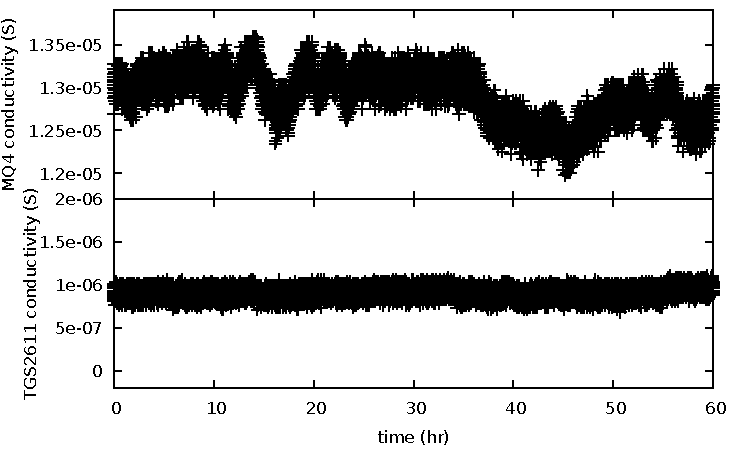
\includegraphics[width=\columnwidth]{honey5.pdf}
				\caption{Long term baseline data were collected at the atmospheric baseline conditions (using a bottle of compressed medical grade breathing air (approximately 0 ppm methane), in the gas mixing chamber.
				%
				The baseline fluctuations can be observed in these plots.}
				\label{fig:MQ4TGSbaseline}
			\end{figure}
			
			Since the initial Fourier analysis showed no significant periodic variations, distribution of the digitized sensor output around the mean response of the sensor was utilized to quantify the precision and baseline noise.
			%
			The data stream (sensor output with time) from each sensor was subtracted from the mean response of the sensor, and a histogram of these differences was created. Since the digitized sensor outputs have a finite number of possible output values, no additional bins were created while producing the analysis.
			%
			Although the data utilized for this analysis were obtained at typical environmental concentrations, additional experiments found that the measured deviation around the mean for each sensor was independent of the concentration of analyte gas.
			%
			There was insignificant correlation between the concentration of the analyte gas and the $\sigma$ obtained at each concentration, as quantified by the Pearson's Correlation Coefficient ($\rho=-0.173$).
			%% PARA
			

			The resulting histograms, along with a best-fit Gaussian peak, are shown in Figs.~\ref{fig:gaussco2}~and~\ref{fig:gaussch4} for the carbon dioxide and methane sensors, respectively.
			%
			In Table~\ref{tab:stddev}, $\sigma_{GAUSS}$ is the standard deviation determine from the Gaussina fit.
			%
			The standard deviation ($\sigma$) calculated from the background subtracted sensor data is almost identical to $\sigma_{GAUSS}$.
			%
			In Figs.~\ref{fig:gaussco2}~and~\ref{fig:gaussch4}, the abscissa (x$-$coordinate) was scaled by the standard deviation of the data set and the area normalized to one.
			%
			The resolution of the dual gas Dynament (MSH-DP/HC/CO2) sensor was insufficient to properly determine the fluctuations around the mean, as this sensor oscillated between two values with time at the given concentration.
			%
			The limited responses is consistent with the resolution stated in their documentation, which lists 0.01\% or 100 ppm as the low end of the concentration range.
			%
			The fluctuation around the mean for the single gas Dynament (MSH-P/CO2) sensor is slightly less that the stated resolution of 50 ppm.
			%% PARA
			
	
			\begin{figure}[!t]
				\centering
				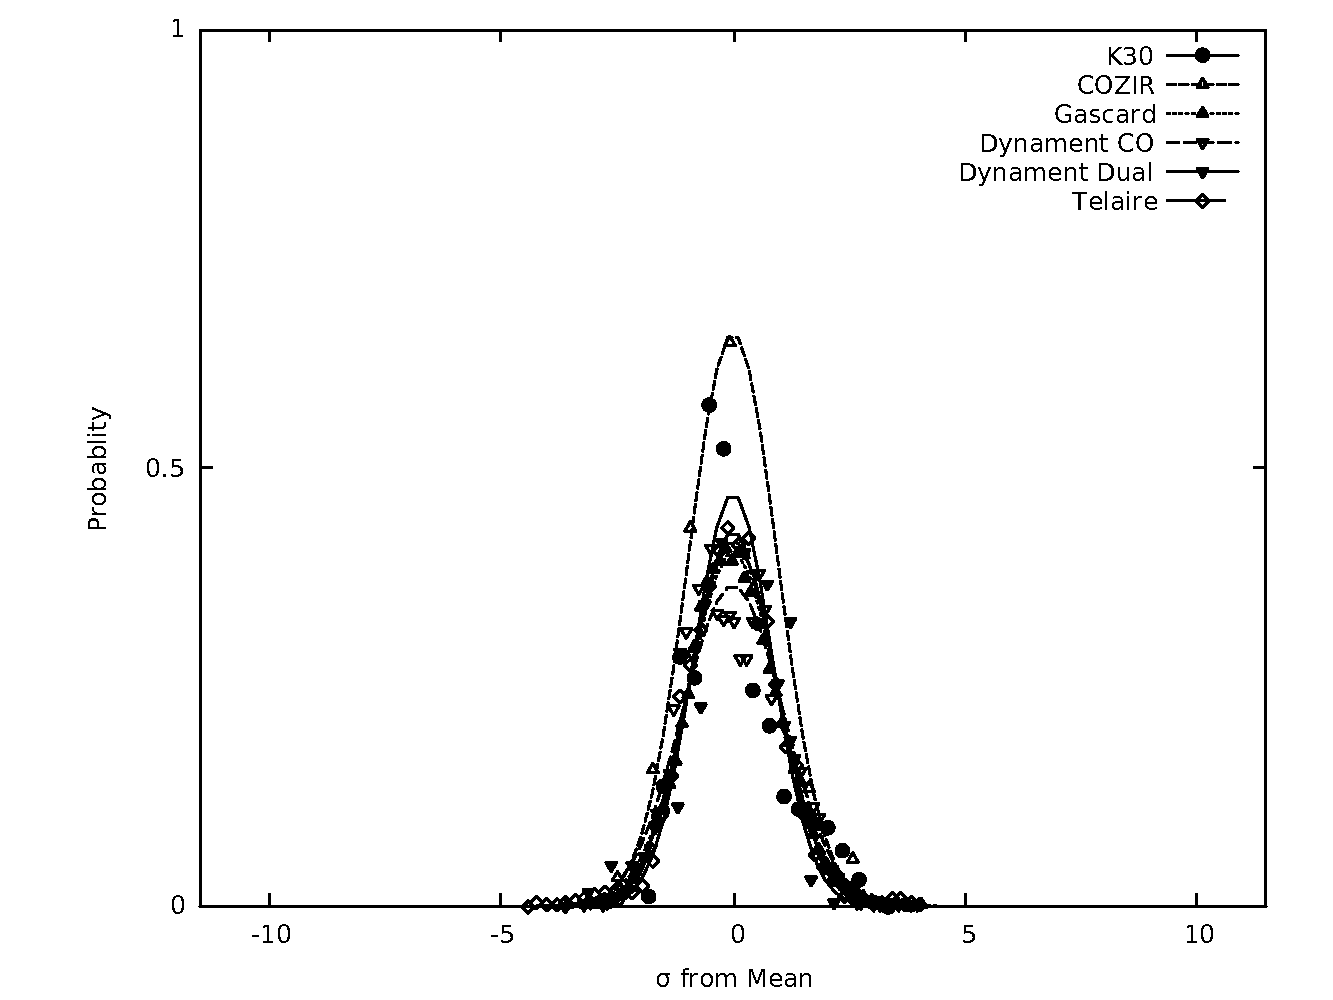
\includegraphics[width=\columnwidth]{honey7.pdf}
				\caption{Frequency distribution of the digitized sensor output around the mean response of the sensor (points), along with Gaussian non-linear for each carbon dioxide sensors around the typical environmental baseline concentration of 400 ppm.
				%
				Any deviation between the center of the Gaussian fit and the mean are due to significant asymmetry of the frequency distribution around the mean.}
				\label{fig:gaussco2}
			\end{figure}
			
			\begin{figure}[!t]
				\centering
				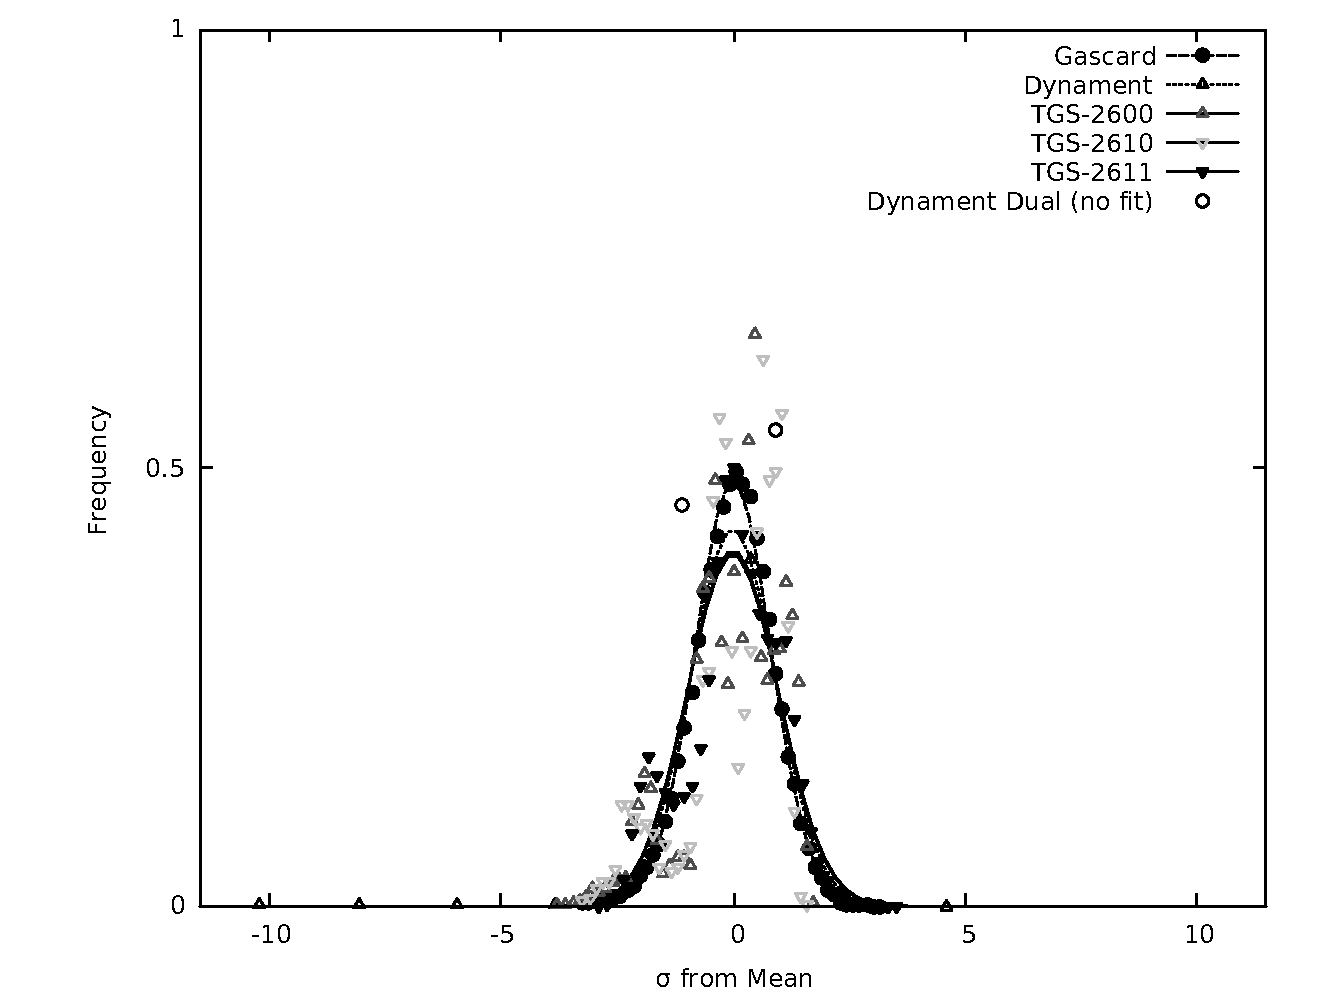
\includegraphics[width=\columnwidth]{honey8.pdf}
				\caption{Frequency distribution of the digitized sensor output around the mean response of the sensor (points), along with Gaussian non-linear fit for each methane sensor around the typical environmental baseline concentration of 0 ppm.
				%
				Any deviation between the center of the Gaussian fit and the mean are due to significant asymmetry of the frequency distribution around the mean.}
				\label{fig:gaussch4}
			\end{figure}
			
			To determine the quality of the Gaussian fits in Figs.~\ref{fig:gaussco2}~and~\ref{fig:gaussch4}, the root-mean-squared error (RMSE) between the fit and the experimentally generated histogram was calculated for each sensor.
			%
			These values are also listed in Table~\ref{tab:stddev}.
			%
			For RMSE, a lower value indicates that the Gaussian function fits closely to the data points, whereas a higher value indicates a poorer fix.
			%
			 The values listed in Table~\ref{tab:stddev} range from roughly 0.150 to 0.300.
			%
			As the probability density function to which the data were fit was normalized to 1, the RMSE values are unitless.
			%
			Since RMSE is a measure of fit, these values can be used in conjunction with $\sigma_{GAUSS}$ to characterize the sensors.
			%% PARA
			
			
			Of the carbon dioxide sensors (see Fig.~\ref{fig:gaussco2} and Table~\ref{tab:stddev}), the Gascard and K-30 sensors produced the smallest standard deviation around the mean, $\sigma_{GAUSS}$, or the highest precision.
			%
			The $\sigma_{GAUSS}$ value of the Telaire sensor was approximately 2 times than that of either the Gascard or the K-30 sensor.
			%
			The COZIR and Dynament (MSH-P/CO2) sensors generated $\sigma_{GAUSS}$ values which were significantly greater than that of the Gascard, Telaire and K-30 sensors.
			%
			Finally, Table~\ref{tab:stddev}) show that the dual gas Dynament (MSH-P/HC/CO2) sensor produced the largest $\sigma_{GAUSS}$ or deviation around the mean. However, the fluctuations around the mean for the Dynament sensors are still lower than the quoted resolutions in the manufacturer's documentation of 50 and 100 ppm, respectively, for these two sensors.
			%% PARA
			
			The Gascard sensor for carbon dioxide produced a normal response around the mean detected value with low RMSE.
			%
			At times, there were some large fluctuations, several standard deviations around the mean response, in the output of the Gascard.
			%
			This suggests that some minimal digital filtering may be required.
			%
			For the K-30 sensor, a good Gaussian fit was produced (small RMSE).
			%
			However, the distribution for the K-30 was skewed toward higher concentration values and appeared to contain two overlapping peaks. This caused the $\sigma_{GAUSS}$ to be slightly larger and the RMSE to be artificially inflated.
			%
			Careful analysis of this double peak showed each peak had a similar standard deviation ($\sigma$), suggesting a small shift in the mean measured value.
			%
			Since the K-30 sensor periodically adjusted for changing backgrounds in the firmware to ensure a normal output concentration of 400 ppm, the observed change in the reported mean concentration in the middle of the run was likely caused by this period background adjustment.
			%
			It is also possible the periodic temperature and pressure variations, which were corrected by the Gascard sensor, were responsible for the observed skew in the K-30.
			%
			In general, precise work requires incorporation of pressure and temperature sensors into potential environmental sensing units to allow ppm corrections to be performed at time of measurement.
			%% PARA
			
			
			The probability distribution of responses around the mean by the GE Telaire sensor is a single peak with a $\sigma_{GAUSS}$ that is approximately 2 to 3 times as large as that of the K-30 and Gascard sensors.
			%
			Since the GE Telaire and K-30 sensor share comparable sensing mechanisms and path lengths, this larger $\sigma_{GAUSS}$ was initially surprising.
			%
			A direct comparison of the response for both the Telaire and K-30 sensors both with and without ambient light, showed that, unlike the K-30 sensor, the Telaire sensor was sensitive to ambient light level.
			%
			Given that long data collection times are required to produce reliable histograms, the ambient light conditions changed over the course of data collection.
			%
			It was suspected that the larger deviations around the mean for the Telaire sensor and resulting $\sigma_{GAUSS}$ values are due to changes in the ambient light.
			%
			Further experiments with the sensor shielded from ambient light confirmed this suspicion.
			%% PARA
			
			
			For the optical methane sensors (see Fig.~\ref{fig:gaussch4} and Table~\ref{tab:stddev}), the Gascard for methane produced a $\sigma_{GAUSS}$ with a low RMSE. The single gas Dynament (MSH-P/HC/) hydrocarbon sensor produced a very low $\sigma_{GAUSS}$ and performed well in terms of precision.
			%
			The $\sigma_{GAUSS}$ for the dual-gas Dynament (MSH-DP/HC/CO2) sensor was not included in this table.
			%
			As mentioned previously, the dual-gas Dynament (MSH-DP/HC/CO2) sensor only reported two values for methane around the mean rather than a distribution of at least several values.
			%
			This result was consistent with the 100 ppm resolution quoted in the manufacturer's documentation for concentrations of less than 10\% methane.
			%% PARA
			

			The result for the chemiresistive methane sensors are also shown in Fig.~\ref{fig:gaussch4}, with a $\sigma_{GAUSS}$ and a RMSE results in Table~\ref{tab:stddev}.
			%
			The distribution curve for the MQ-4 sensor was not included.
			%
			Since the MQ-4 sensor displayed significant baseline drift when compared to the TGS-2611 sensor (Fig.~\ref{fig:MQ4TGSbaseline}), the standard deviation was instead calculated directly from a relatively flat region of the baseline.
			%
			This different treatment was not inconsistent with the use of the sensor in many applications where drift is a result of temperature and humidity.
			%
			 In general, the use of a dynamic background subtraction algorithm is required for chemiresistive sensors.
			%
			The $\sigma_{GAUSS}$ results of the TGS-2600 and TGS-2610 were similar, as expected due to their similar sensing mechanisms.
			%
			The baseline noise, as quantified by $\sigma_{GAUSS}$, for the methane optimized TGS-2611 sensor was lower than the other TGS sensors.
			%% PARA
			
			
			\begin{table}[!t]
				\begin{center}
					\begin{threeparttable}
						\renewcommand{\arraystretch}{1.3}
						\caption{The first two numbered are the computed standard deviation in ppm of Gaussian fitted probability distributions and root-mean-squared error in the fit.
						%
						The next two numbers are the computed IUPAC ($3\sigma_{GAUSS}$) and calibration uncertainty corrected Limits of Detections in ppm.}
						\label{tab:stddev}
						\begin{tabular}{ c | r | c c c c }
							& Sensor & $\sigma_{GAUSS}$ (ppm) & RMSE & IUPAC & Corrected\tnote{\dag}   \\ \hline
							\multirow{6}{*}{\rotatebox[origin=c]{90}{Carbon Dioxide}}
							& K-30 SE-0018     & 1.91   & 0.219  & 5.7 & 27.1\\
							& COZIR AMB GC-020 & 14.1   & 0.304 & 42.3  & 80.6\\
							& Gascard CO$_2$   & 2.12   & 0.223 &  6.4 & 32.1\\
							& MSH-DP/HC/CO2   & 86.4   & 0.197  & 260 & 254\\
							& MSH-P/CO2       & 17.6   & 0.217 & 52.8 & 68.0\\
							& Telaire T6615    & 4.42   & 0.185 & 13.3 & 31.1\\ \hline
							\multirow{4}{*}{\rotatebox[origin=c]{90}{Methane/Hydrocarbon}}
							& MQ-4  & 26.7 \tnote{\ddag}  & & 80.0 & 82.0\\
							& Gascard CH$_4$   & 35.7   & 0.222  & 110 & 151\\
							%& MSH-DP/HC/CO2   &see text&see text  \\
							& MSH-P/HC       & 3.54   & 0.152  & 10.6 & 170 \\
							& TGS-2600         & 36.1   & 0.225  & 110 & 117 \\
							& TGS-2610         & 37.1   & 0.237  & 111 & 113 \\
							& TGS-2611         & 5.4  & 0.208 & 16.3 & 16.3
						\end{tabular}
						\begin{tablenotes}
							\vspace{3pt}
							\item[\dag] A linear calibration was utilized for the optical sensor, while the chemiresistive utilized the non-linear Langmuirian fit. See text.
							\item[\ddag] This value was determined directly from the experimental response.
							%
							See text.
							\vspace{1eX}
						\end{tablenotes}
					\end{threeparttable}
				\end{center}
			\end{table}
			
		\subsection{Limits of Detection}	
	
			The limits of detection were determined as discussed in Section~\ref{sec:method_detection} and are listed in Table~\ref{tab:stddev}.
			%
			It should be noted these tests were carried out in a controlled environment and are best-case values.
			%
			Of the tested carbon dioxide sensors, the Gascard, K-30, and Telaire sensors have comparable low Limits of Detection.
			%
			The COZIR and Dynament single analyte sensor (MSH-P/CO2) have the next highest Limit of Detection, and the Dynament dual analyte sensor (MSH-DP/HC/CO2) has the highest.
			%
			These results reflect the ordering of $\sigma_{GAUSS}$ in Table~\ref{tab:stddev}. They can be correlated with the optical path lengths of the sensors, in which larger pathways resulting in greater sensitively.
			%% PARA
			
		
			The Limit of Detection for the Dynament single analyte methane sensor (MSH-P/HC)demonstrates the important influence of calibration error on the reported limit.
			%
			For this sensor, the 3.54 ppm precision ($\sigma_{GAUSS}$) or deviation around the mean was significantly lower than the 50 ppm resolution quoted in the manufacturer's documentation at the low-end of the 1\% concentration range of the sensor.
			%
			Given the 50 ppm resolution, an IUPAC Limit of Detection of at least 150 ppm would be expected. After correcting for the calibration error, the Limit of Detection is 170 ppm, consistent with expectations.
			%
			However, the value produced by directly applying IUPAC $3\sigma$ definition was 16 times lower, illustrating the necessity of including the calibration uncertainty.
			%% PARA
			
	
			Of the tested chemiresistive methane sensors, the TGS-2611 sensor had the lowest Limit of Detection under controlled conditions, primarily due to its stable baseline, which influences both the background noise and the quality of the calibration.
			%
			Similar sensitivities have been reported for the TGS-2600~\cite{eugster_performance_2012}.
			%
			Both the non-methane optimized TGS-2600 and TGS-2610 sensors had similar limits of detection which were slightly larger than the methane optimized TGS-2611 and the MQ-4.
			%
			The MQ-4 sensor has precision between the TGS-2611 and both the TGS-2600 and TGS-2610 sensors.
			%
			The 82 ppm limits of detection for the MQ-4 sensor is consistent with scatter in the calibration curve at concentration under 100 ppm (see Fig.~\ref{fig:mq4step}).
			%% PARA
			
			
			\FloatBarrier	
	
	\section{Conclusion}
	
		The performance of a sensor platform for environmental or industrial monitoring is sensitive to the cost and performance of the individual sensor elements.
			%
			Thus, the detection limits, accuracy, and precision for a range of potential sensors for measuring ppm concentrations of carbon dioxide and methane for low-cost monitoring instrumentation were quantified.
			%
			These parameters were quantified around the baseline atmospheric concentration for each analyte gas, which is approximately 400 ppm for carbon dioxide~\cite{blasing_recent_2016,dlugokencky_trends_2016} and under 2 ppm for methane~\cite{turner_large_2016,bamberger_spatial_2014,dlugokencky_trends_2016-1}.
			%
			The selected sensors were also evaluated at gas concentrations exceeding 1000 ppm, in order to mimic a leak.
			%% PARA
			
		
		For carbon dioxide, the Gascard sensor had high performance based on the low errors reported in Table~\ref{tab:stddev}, but is comparatively more expensive than the other sensors investigated.
		%
		The Gascard is limited by reliance on active sampling, which requires a pump that introduces a source of additional power consumption, a mechanical failure point, and sampling complexity.
		%
		Since concentrations are parts-per notation, the inclusion of temperature and pressure corrections on the Gascard is useful to automatically correct for these values.
		%
		Thus, this sensor eliminates the need for additional sensors for precise measurements.
		%
		 Both the K-30 and Telaire sensors had good performance.
		%
		The ability of the K-30 and Telaire sensors to operate by passive diffusion rather than mechanically pumped flow also reduces the cost and complexity of a potential monitoring system.
		%
		 The K-30 sensor also has the option to autozero by assuming the minimum concentration of a multi-day run is 400 ppm, if used properly, this feature has advantages for remote instrumentation.
		%% PARA
		
		
		For methane, there is no single sensor which meets the ppm or even sub-ppm sensitivity required for environmental monitoring. The Limit of Detection for the selected relativity low-cost optical methane sensors reported in Table~\ref{tab:stddev}, collectively show that these NDIR sensors are not suitable for monitoring environmental levels of methane around the global average.
		%
		Although progress has been made to produce viable sensors~\cite{zhu_one_2012}, larger, more costly devices are still required for precision measurements at the ppm level.
		%
		With an increasing focus on remote sensing technology, more precise low-cost methane sensors are required to produce accurate data at expected atmospheric concentrations.
		%
		This work provides a framework for future sensor developers to follow to provide performance results in a manner which faithfully compares them to existing devices.
		%% PARA
		
	
	%%%%%%%%%%%%%%%%%%%%%%%%%%%%%%%%%%%%%%%%%%
	\authorcontributions{Conceptualization, X.X. and Y.Y.; methodology, X.X.; software, X.X.; validation, X.X., Y.Y. and Z.Z.; formal analysis, X.X.; investigation, X.X.; resources, X.X.; data curation, X.X.; writing--original draft preparation, X.X.; writing--review and editing, X.X.; visualization, X.X.; supervision, X.X.; project administration, X.X.; funding acquisition, Y.Y.}
	
	%%%%%%%%%%%%%%%%%%%%%%%%%%%%%%%%%%%%%%%%%%
	\funding{%
		The authors acknowledge the financial support of this work by U.S. Department of Energy under contract DE-FOA-0000798.
		%
		Additional support was provided by Oklahoma State University.
	}%
	
	%%%%%%%%%%%%%%%%%%%%%%%%%%%%%%%%%%%%%%%%%%
%	\acknowledgments{In this section you can acknowledge any support given which is not covered by the author contribution or funding sections. This may include administrative and technical support, or donations in kind (e.g., materials used for experiments).}
	
	%%%%%%%%%%%%%%%%%%%%%%%%%%%%%%%%%%%%%%%%%%
	\conflictsofinterest{The authors declare no conflict of interest.} 
	
	%%%%%%%%%%%%%%%%%%%%%%%%%%%%%%%%%%%%%%%%%%
	%% optional
	\abbreviations{The following abbreviations are used in this manuscript:\\
		
	\noindent 
	\begin{tabular}{@{}ll}
			\ce{CO2} & Carbon dioxide\\
			\ce{CH4} & Methane\\
			TLA & Three letter acronym\\
			LD & linear dichroism
	\end{tabular}}
	
%	\bibliographystyle{elsarticle-num}
	\externalbibliography{yes}
	\bibliography{bib}
	
\end{document}



